% !TEX root = ../../main.tex

\subsection{A study on a novel MOF}

With the methods of characterisation through calorimetry
outlined on a reference material, a similar study on a 
MOF sample can be performed. The aim is to screen for 
potentially interesting features for use in gas 
storage and separation.

\subsubsection{Material}

Zr Fumarate, also known as MOF-801, is a fumaric 
acid analogue of the well-known UiO-66(Zr) 
framework~\cite{wissmannModulatedSynthesisZrfumarate2012}.
Its structure is similar to that of UiO-66, although 
the smaller non-linear linker leads to a lowering of 
symmetry and a slight tilting in the Zr-O clusters,
as depicted in \autoref{calo:fgr:zrfum-structure}.
The MOF is synthesised using the modulated synthesis method and 
formic acid as the modulator to increase the crystalinity of the
material. Indeed, when not using this approach, the resulting
material is nearly amorphous~\cite{zahnInsightMechanismModulated2014}.
In this study the sample was synthesised according to the procedure 
detailed in \autoref{appx:synthesis:zrformate}.

\begin{figure}[htb]
    \centering
    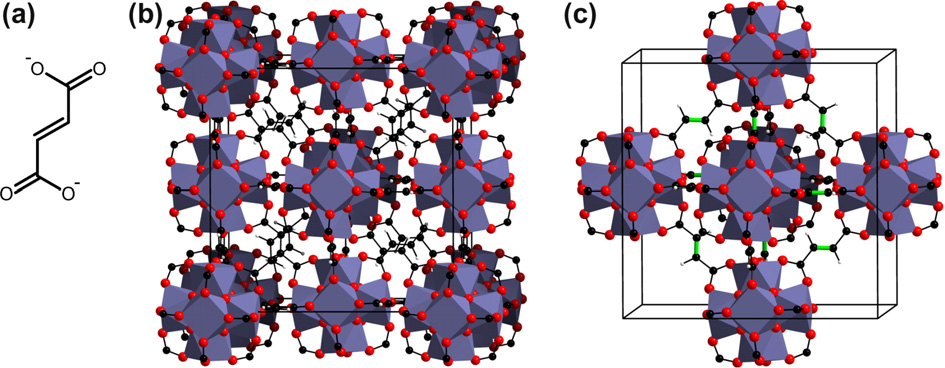
\includegraphics[width=0.8\textwidth]{zrfum/structure}%
    \caption{(a) The fumarate linker used in the Zr Fumarate
    MOF, an ionic form of \textit{trans}-butenedioic acid and
    (b) and (c) the structural model of the MOF. Illustration
    adapted from~\citeauthor{wissmannModulatedSynthesisZrfumarate2012}%
    \cite{wissmannModulatedSynthesisZrfumarate2012}.}%
    \label{calo:fgr:zrfum-structure}
\end{figure}

Zr Fumarate has recently been the subject of interest due to its
high water stability~\cite{zahnWaterbornZrbasedPorous2015}, 
as well as its potential to be synthesised through green synthesis
routes~\cite{reinschFacileGreenRoute2016} or direct
monolith formation with a gel approach~\cite{buekenGelbasedMorphologicalDesign2017}.

Furthermore, the material has a remarkably steep water adsorption
behaviour at low pressure~\cite{furukawaWaterAdsorptionPorous2014},
which has led to its possible application as a water scavenger 
membrane~\cite{baeTransparentMetalOrganic2016} or in a water 
harvesting device which would capture water from air in low relative
humidity environments such as the desert. While initial 
attempts~\cite{kimWaterHarvestingAir2017} were criticised for
overpromising performance, more recent modifications to such 
a system have addressed some of these 
concerns~\cite{kimAdsorptionbasedAtmosphericWater2018}.

The low relative pressure of water adsorption has highlighted
the contribution of defects~\cite{choiRoleStructuralDefects2018} in 
shifting the adsorption isotherm, an effect arising from cooperative
interactions and initial clustering of water molecules on defect
sites~\cite{vandichelWaterCoordinationDehydration2016}.

As the properties of the MOF diverge from the ideal properties
indicated by the structure, an experimental study to test for the adsorption
or separation of other molecules may reveal unexpected 
applications.

\subsubsection{Results}

Adsorption isotherms of nine probe gasses were recorded at 
\SI{303}{\kelvin} through combined manometry and microcalorimetry
as described in \autoref{calo:method:calo}. The complete 
dataset can be seen in \autoref{calo:fgr:zrfum-data}.

\begin{figure}[htb]
    \centering

	\begin{subfigure}[b]{.45\textwidth}
        \centering
        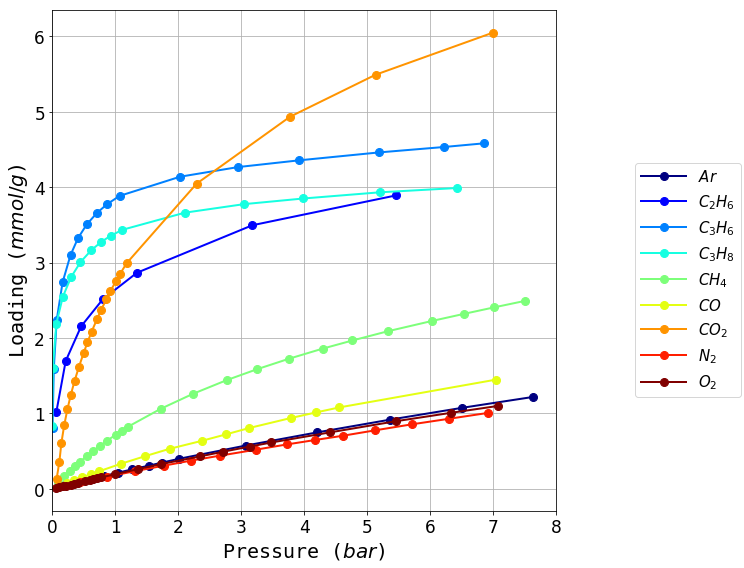
\includegraphics[width=\linewidth]{zrfum/zrfum-dataset}
        \caption{}%
        \label{calo:fgr:zrfum-dataset}
    \end{subfigure}%
	\quad
	\begin{subfigure}[b]{.45\textwidth}
        \centering
        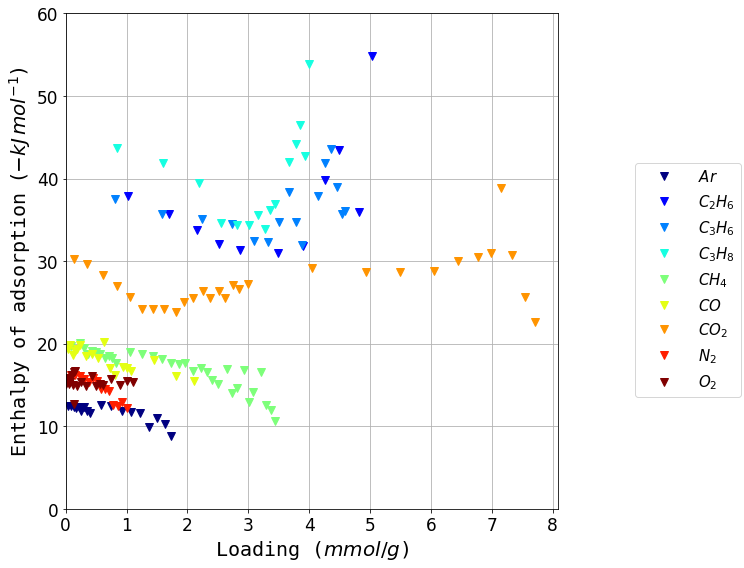
\includegraphics[width=\linewidth]{zrfum/zrfum-enthalpy}
        \caption{}%
        \label{calo:fgr:zrfum-enthalpy}
    \end{subfigure}
    \caption{(a) The experimental isotherms of all recorded gases and
    (b) the corresponding enthalpy curves.}%
    \label{calo:fgr:zrfum-data}

\end{figure}



Values for initial Henry's constant and initial enthalpy of adsorption
were calculated using the methods available in pyGAPS.
The same trend as with the Takeda 5A sample was plotted in 
\autoref{calo:fgr:zrfum-trends}. 

\begin{figure}[htb]
    \centering

    \begin{subfigure}[b]{0.5\textwidth}
        \centering
        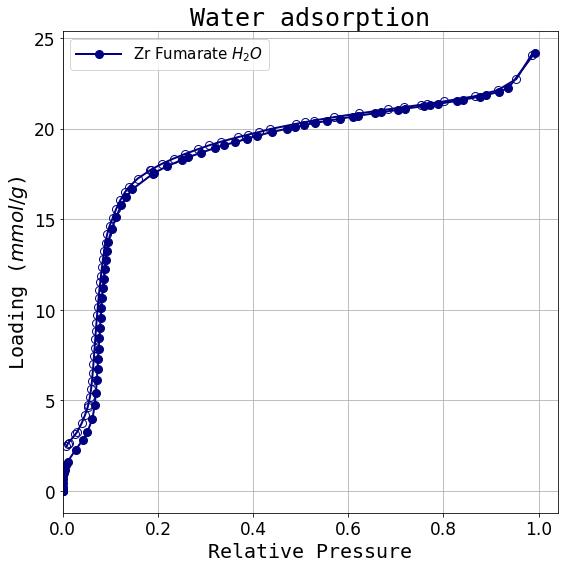
\includegraphics[width=\linewidth]{zrfum/zrfum-water}
        \caption{}%
        \label{calo:fgr:zrfum-water}
    \end{subfigure}%
    \begin{subfigure}[b]{0.5\textwidth}
        \centering
        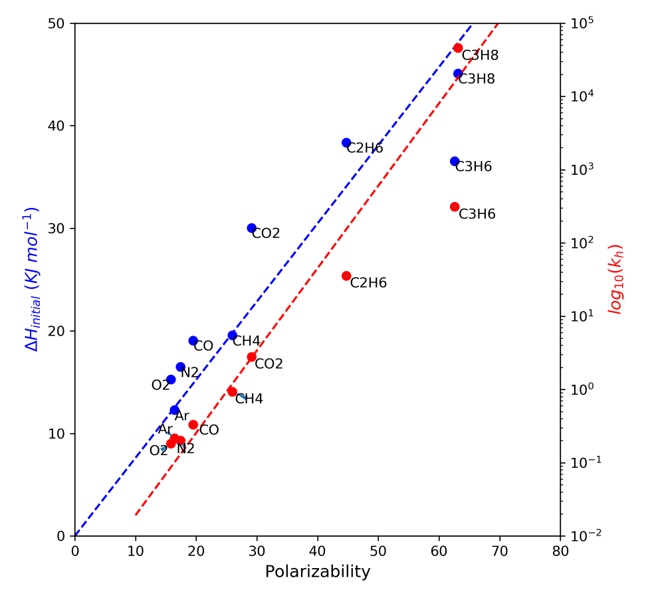
\includegraphics[width=\linewidth]{zrfum/zrfum-enth-henry}
        \caption{}%
        \label{calo:fgr:zrfum-trends}
    \end{subfigure}
    \caption{(a) The experimental dataset all recorded gases and
    (b) the calculated trends of initial heat of adsorption (red) and 
    Henry's constant (blue). The dotted lines are best fit lines to 
    the series of unsaturated hydrocarbons.}%
    \label{calo:fgr:zrfum-analysis}

\end{figure}